\documentclass[border=4pt]{standalone}
\usepackage[T1]{fontenc}
\usepackage{mathptmx}
\usepackage{xcolor}
\usepackage{tikz}
\usetikzlibrary{positioning,arrows.meta,calc,fit,backgrounds}
\definecolor{lugar}{HTML}{CDE2FB}
\definecolor{atrator}{HTML}{F6C9B5}
\definecolor{tinta}{HTML}{3B3B38}
\definecolor{azul}{HTML}{2A78D6}
\definecolor{laranja}{HTML}{EB6834}
\begin{document}
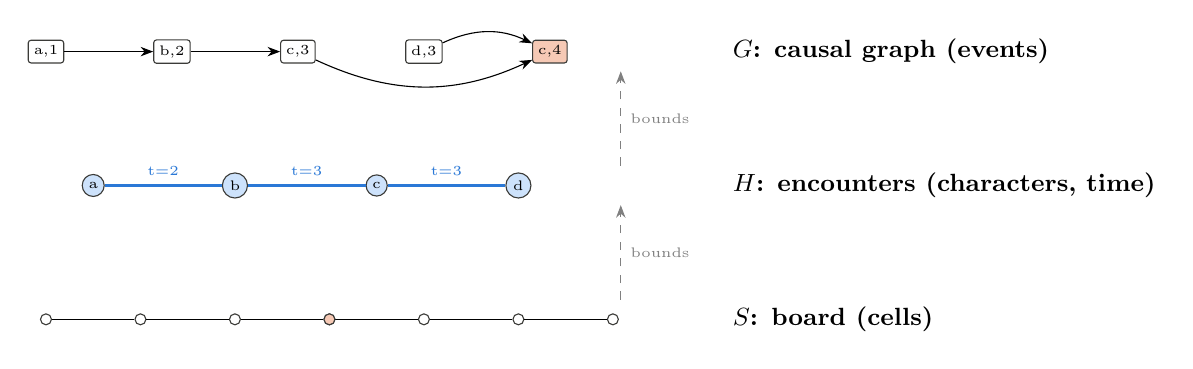
\begin{tikzpicture}[
  no/.style={circle,draw=tinta,fill=white,inner sep=1.4pt},
  ev/.style={rectangle,rounded corners=1pt,draw=tinta,fill=white,inner sep=2pt,font=\tiny},
  cam/.style={font=\small\bfseries,anchor=west},
  >={Stealth[length=1.6mm]}]
  % camada 1: espaço
  \begin{scope}[yshift=0cm]
    \foreach \i in {0,...,6} \node[no] (s\i) at (\i*1.2,0) {};
    \foreach \i [evaluate=\i as \j using int(\i+1)] in {0,...,5} \draw (s\i) -- (s\j);
    \node[no,fill=atrator] at (s3) {};
    \node[cam] at (8.6,0) {$S$: board (cells)};
  \end{scope}
  % camada 2: encontros
  \begin{scope}[yshift=1.7cm]
    \foreach \i/\x in {a/0.6,b/2.4,c/4.2,d/6.0} \node[no,fill=lugar] (h\i) at (\x,0) {\tiny\i};
    \draw[azul,thick] (ha) -- node[above,font=\tiny]{t=2} (hb);
    \draw[azul,thick] (hb) -- node[above,font=\tiny]{t=3} (hc);
    \draw[azul,thick] (hc) -- node[above,font=\tiny]{t=3} (hd);
    \node[cam] at (8.6,0) {$H$: encounters (characters, time)};
  \end{scope}
  % camada 3: eventos
  \begin{scope}[yshift=3.4cm]
    \node[ev] (e1) at (0,0) {a,1};
    \node[ev] (e2) at (1.6,0) {b,2};
    \node[ev] (e3) at (3.2,0) {c,3};
    \node[ev] (e4) at (4.8,0) {d,3};
    \node[ev,fill=atrator] (e5) at (6.4,0) {c,4};
    \draw[->] (e1) -- (e2);
    \draw[->] (e2) -- (e3);
    \draw[->,bend left=25] (e4) to (e5);
    \draw[->,bend right=25] (e3) to (e5);
    \node[cam] at (8.6,0) {$G$: causal graph (events)};
  \end{scope}
  \draw[->,gray,dashed] (7.3,0.25) -- node[right,font=\tiny,text=gray]{bounds} (7.3,1.45);
  \draw[->,gray,dashed] (7.3,1.95) -- node[right,font=\tiny,text=gray]{bounds} (7.3,3.15);
\end{tikzpicture}
\end{document}
